In this chapter, we will take closer look on the programming language Java. We will primarily focus on description of its division into platforms and distribution, which will be important for comparison with Android API later. 
%V této kapitole si stručně popíšeme programovací jazyk Java. Zaměříme se především na popis jeho rozdělení do platforem a distribucí.

\section{Java}
Java \cite{JavaBook} is one of the most used and most famous computer programming languages in the world. It's developed as opensource by Oracle Corporation and the syntax of this language belongs to those simpler, but its application is very widespread. Java is used for programming smart cards, mobile and desktop applications, as well as large business and information systems. Java is multiplatform language therefore it can easily be ported on different operating systems.  
%Java je jedním z nejpoužívanějších a nejpopulárnějších počítačových programovacích jazyků na světě. Syntaxe tohoto jazyka se řadí k těm jednodužším, avšak jeho použití je velmi rozsáhlé. V Java se programují čipové karty, mobilní a desktopové aplikace, i velké podnikové a informační systémy. Java je jazyk multiplatformní a díky tomu je jej možné použít ná různých operačních systémech. Java je vyvíjena jako OpenSource. Java se objevuje ve třech základních edicích:

\subsection{Java platforms}
Java language is published in four platforms. Every platform has own specific designation. In this section we will briefly describe these platforms.
%Jazyk Java je společně s virtuálním strojem a knihovnami vydáván ve čtyřech platformách, kde každá má své speciální určení.

\subsubsection{Java Standard Edition (Java SE)}
Basic and the most famous platform, which is designed for development of desktop and simpler server application. Currently, the most recent version is Java SE 8.
%Základní platforma pro vývoj desktopových a jednodužších serverových aplikací. V součané době je poslední vydaná verze Java SE 8u25.

\subsubsection{Java Enterprise Edition (Java EE)}
Java EE is extension of Java SE that contains special libraries for developing and running enterprise software applications and information systems. Java EE in current version is based on Java SE 7.
%Nádstavba nad Java SE obsahující speciální knihovny pro vývoj a provoz podnikových aplikací a informačních systémů. V součané době je poslední vydaná verze Java EE 7.

\subsubsection{Java Micro Edition (Java ME)}
Java ME is subset of Java SE for application development for small devices such as microcontrolers, mobile phones, set-top boxes, printers and others. Currently, the most recent version is Java ME 8.1.
%Podmnožina Java SE pro vývoj aplikací pro malá zařízení jako jsou mikrokontroléry sensory, mobilní telefony, set-top boxy, tiskárny a další. V součané době je poslední vydaná verze Java ME 8.1.

\subsubsection{Java Card}
Java Card is technology designed for application development for smart card and devices with limited memory and processing capabilities. For example, it is used for SIM cards for mobile devices, plastic smart card for ATM and other devices. Last released version is Java Card 3.
%Verze určená pro vývoj aplikací určených pro čipové karty a pro zařízení s limitovanou pamětí a schopností zpracovávání. Příkladem mohou být SIM karty pro mobilní zařízení nebo čipové karty pro ATM bankomaty. V součané době je poslední vydaná verze Java Card 3.0.4.

\subsection{Java SE distributions}
Let's take a closer look at the Java SE. There are two distributions of Java SE platform: Java JRE -- the running environment and JDK -- the development tool. Figure \ref{jdk} shows parts of JDK distributions in comparison with JRE.
%Možnosti jak Javu stáhnout jsou dvě. Jedná se o balík se kterým lze pouze spouštět aplikace Java (JRE) nebo balík který slouží pro vývoj (JDK).

\subsubsection{Java SE Runtime Environment (JRE)}
JRE is runtime environment to run applications written in Java programming language. It consist from Java API, Java virtual machine, tool for creating rich internet applications (JavaFX) and deployment tools.
%Běhové prostředí Javy, které poskytuje vše potřebné pro suštění java aplikací. Součástí je virtuální stroj javy a potřebné knihovny.

\subsubsection{Java SE Development Kit (JDK)}
Java SE Development Kit is sometimes known as Software Development Kit (SDK). It includes JRE plus development tools such as compiler, documentation generator, debubers and other tools.
%Někdy se také označuje SDK (Software Development Kit). Jedná se o sadu JRE doplněnou o vyvojářské nástroje (překladač, generátor dokumentace, ladící nástroje a další).
\\
\begin{figure}[h!]
    \centering
    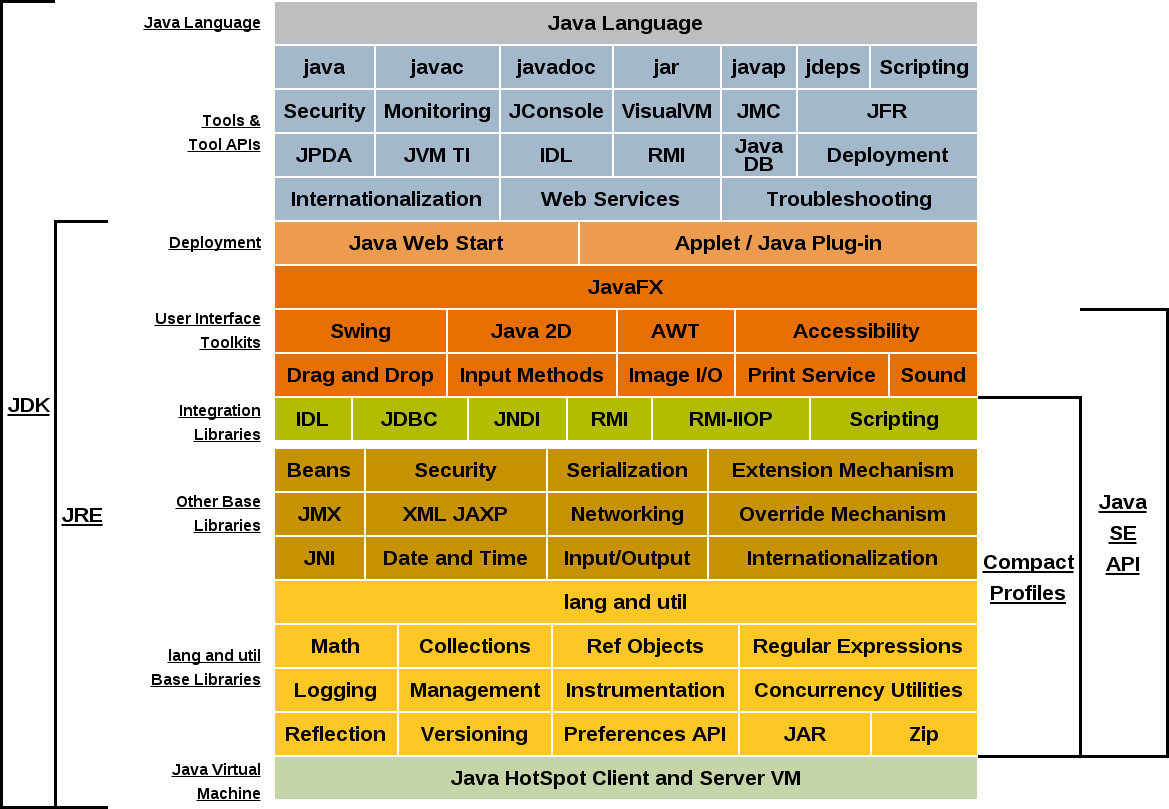
\includegraphics[scale=0.35]{fig/java_jdk.jpg}
    \caption{Java SE JDK 1.8 \cite{Java8Doc}}
    \label{jdk}
\end{figure}

%\subsection{History}
%V následující tabulce je stručně popsána historie programovacího jazyku Java: \\
%\\
%\begin {table}[h!]
%\begin{tabular}{|l|l|l|}[h]
%\hline
%    {\bf Název} & {\bf Datum} & {\bf Poznámka}  \\
%    \hline \hline
%    Oak         & 1991                  & a     \\
%    JDK         & 1995                  & a     \\
%    JDK 1.0     & January 23rd, 1996    & a     \\
%    JDK 1.1     & February 19th, 1997   & a     \\
%    JPE         & May, 1998             & a \\
%    J2SE 1.2    & December 8th, 1998    & a     \\
%    J2EE 1.2    & December 12, 1999     & a     \\
%    J2SE 1.3    & May 8th, 2000         & a     \\
%    J2EE 1.3    & September 24, 2001    & a \\
%    J2SE 1.4    & February 6th, 2002    & a     \\
%    J2EE 1.4    & November 11, 2003     & a \\
%    J2SE 5.0    & September 30th, 2004  & a     \\
%    Java EE 5   & May 11, 2006          & a \\
%    Java SE 6   & December 11th, 2006   & a     \\
%    Java EE 6   & December 10, 2009     & a \\
%    Java SE 7   & July 28th, 2011       & a     \\
%    Java EE 7   & June 12, 2013         & a \\
%    Java SE 8   & March 18th, 2014      & a     \\
%  \hline
%\end{tabular}
%\caption{Historie Javy}
%\end{table}

